\section{Interfaz}

La interfaz de usuario desarrollada para el UAV de ala fija incluye varios componentes que permiten una visualización integral de los parámetros de vuelo y el estado de la aeronave en tiempo real. Los parámetros considerados más cruciales se han incorporado en diferentes secciones de la interfaz, facilitando el monitoreo y el control efectivo del UAV. A continuación se describen estos componentes:

\subsection{Mapa de Posición en Tiempo Real}

En la figura \ref{fig:mapa Interfaz } se puede observar un apartado en el que se observa la posición del UAV en tiempo real utilizando un mapa interactivo. La posición actual se muestra con coordenadas de latitud y longitud, permitiendo un seguimiento preciso del UAV durante su vuelo.

\begin{figure}[H]
    \centering
    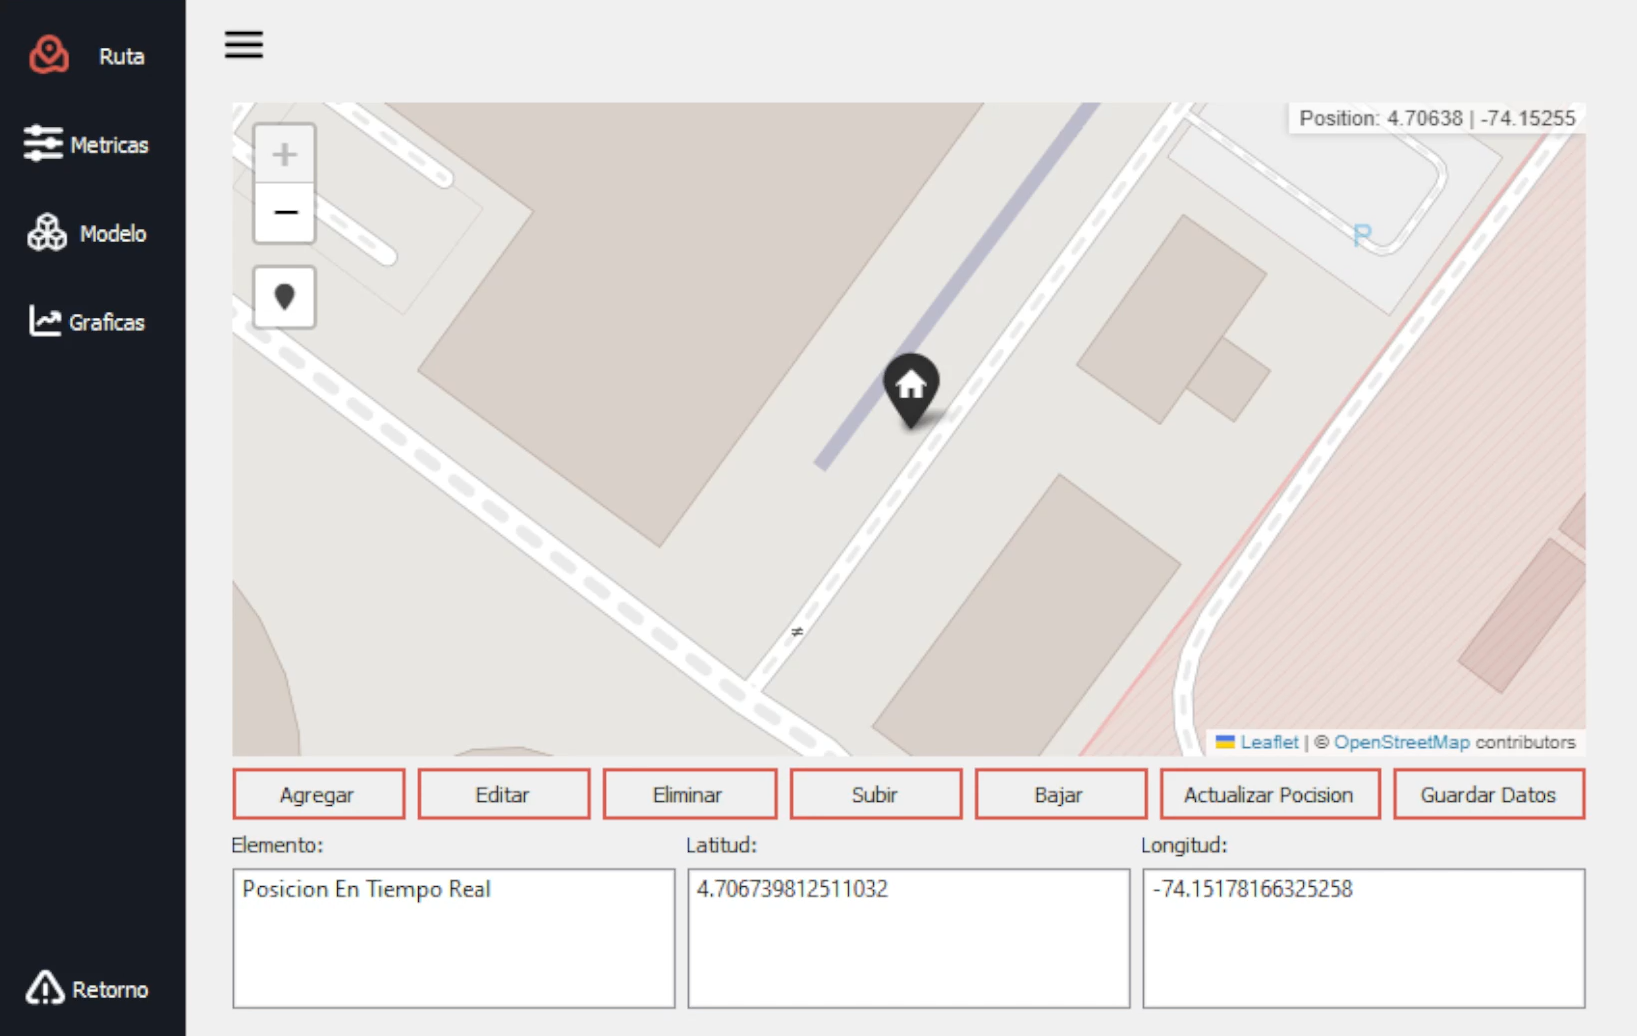
\includegraphics[width=6 in]{Imagenes/Interfaz/mapa_interfaz.png}
    \caption{Mapa de Visualización UAV}
    \label{fig:mapa Interfaz }
\end{figure}

\subsection{Indicadores de Vuelo:}

Las indicadores de vuelo se presentan mediante instrumentos de control similares a los que se encuentran en una aeronave real (véase \ref{fig:metricas interfaz }). Estos instrumentos incluyen:
\begin{itemize}
    \item \textbf{Horizonte Artificial:} Indica la actitud del avión en términos de yaw, pitch y roll.
\item \textbf{Altímetro:} Mide la altitud del UAV con referencia a la altitud inicial del dispositivo.
\item \textbf{Barómetro:}Indica la presión atmosférica.
\item \textbf{Airspeed: }Mide la velocidad del aire.
\item \textbf{Manifold Pressure:} Muestra la presión del colector, relevante para el rendimiento del motor.
\end{itemize}

\begin{figure}[H]
    \centering
    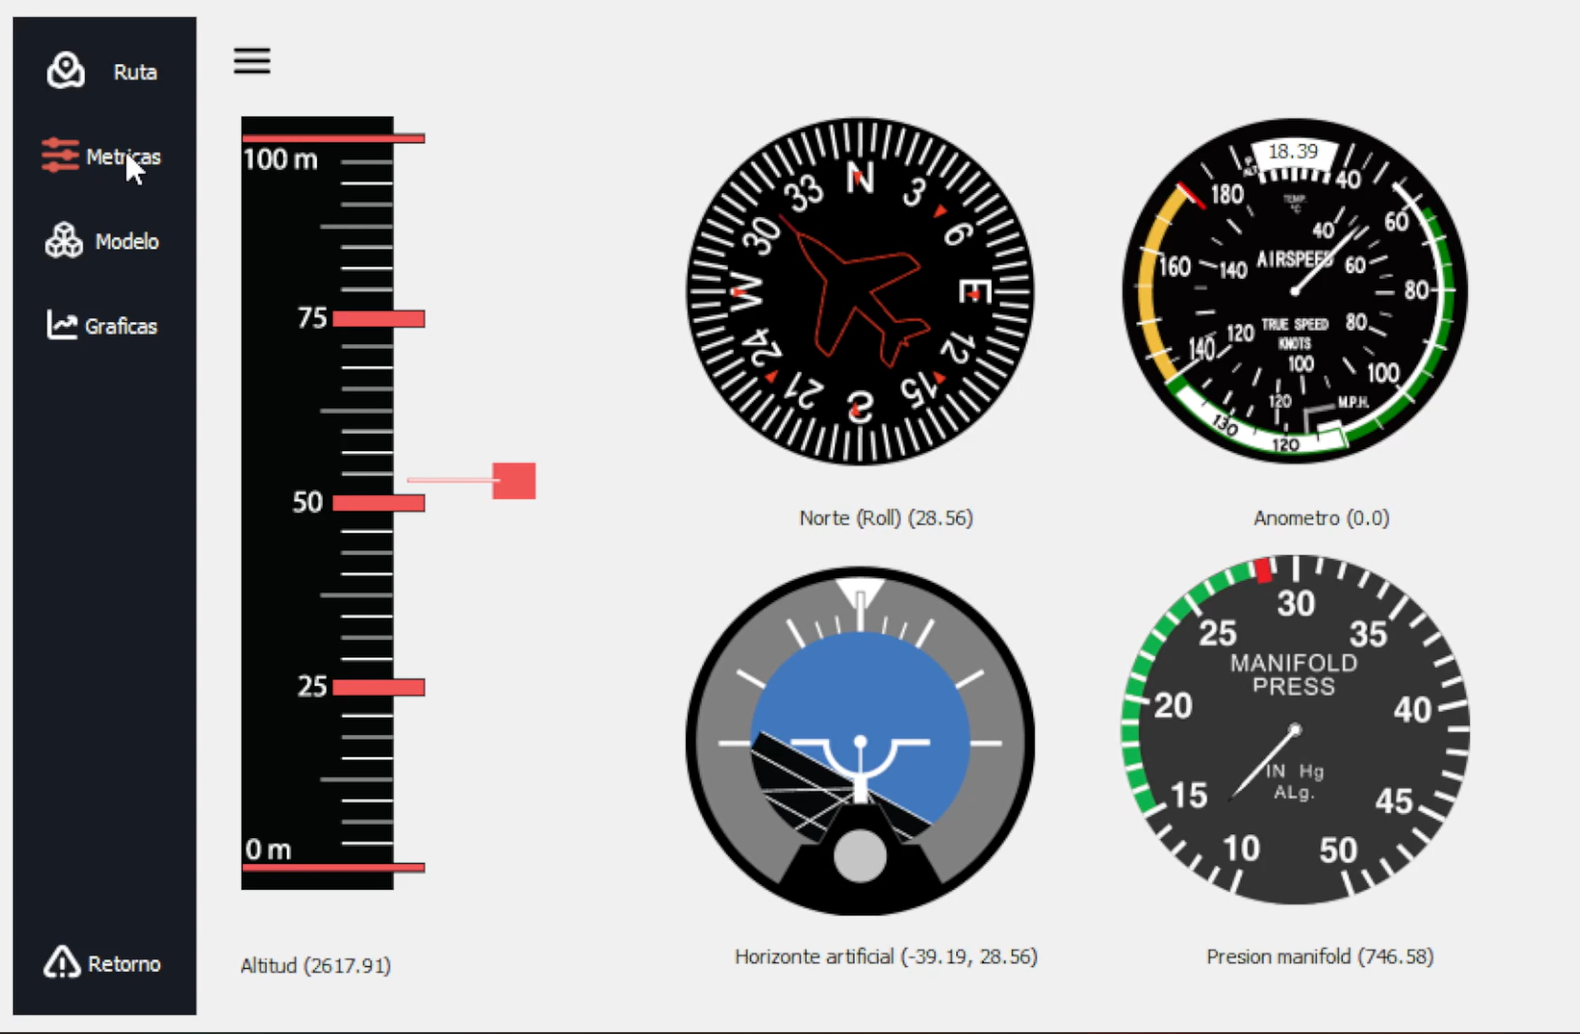
\includegraphics[width=6 in]{Imagenes/Interfaz/metricas.png}
    \caption{indicadores de vuelo para un UAV}
    \label{fig:metricas interfaz }
\end{figure}

\subsection{Modelo 3D del UAV:}

Se incluye un modelo tridimensional del UAV que representa su orientación en el espacio \ref{fig:modelo 3d inerfaz }.  Proporcionando una visualización clara de la dirección hacia donde está apuntando el UAV, facilitando la comprensión de su comportamiento dinámico.
\begin{figure}[H]
    \centering
    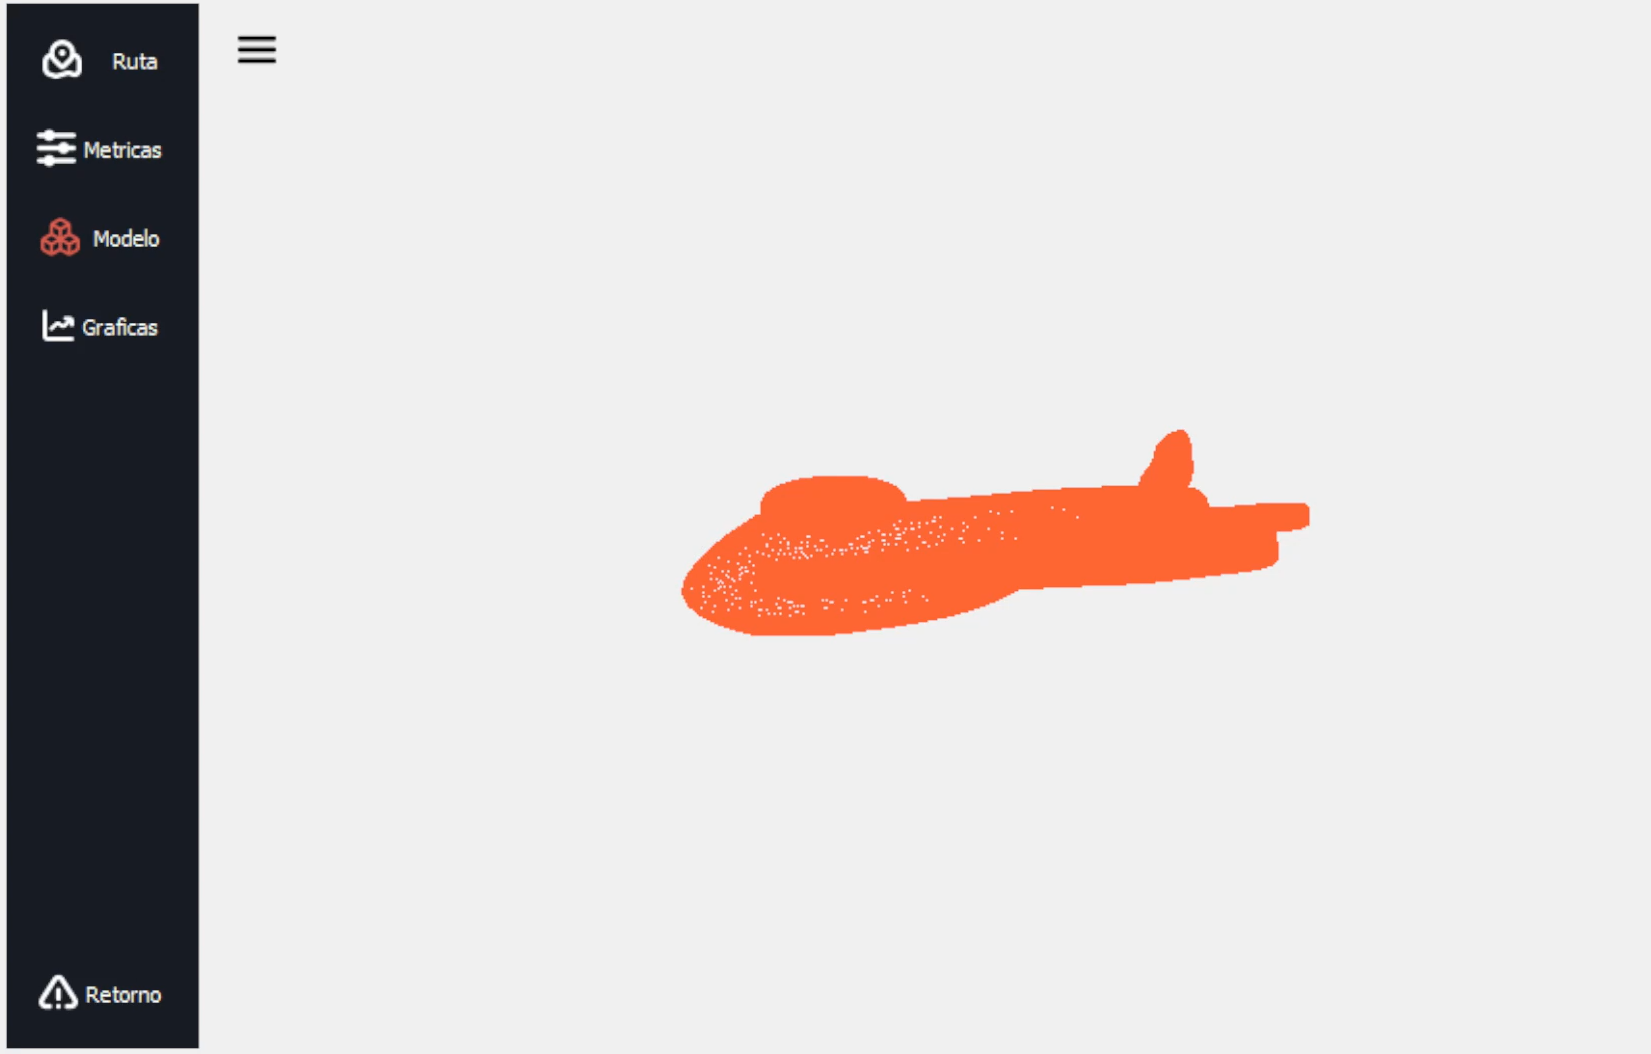
\includegraphics[width=5 in]{Imagenes/Interfaz/modelo3d.png}
    \caption{Modelo 3d UAV en la Interfaz}
    \label{fig:modelo 3d inerfaz }
\end{figure}

\subsubsection{Gráficas en Tiempo Real:}

Esta sección permite visualizar diferentes comportamientos históricos de la aeronave. Las gráficas muestran datos como movimientos inerciales (roll, pitch, yaw), altitud, temperatura, presión, y velocidad en función del tiempo. Estas gráficas son cruciales para analizar y evaluar el rendimiento del UAV durante vuelo para observar y analizar el comportamiento histórico de la aeronave.

\begin{figure}[H]
    \centering
    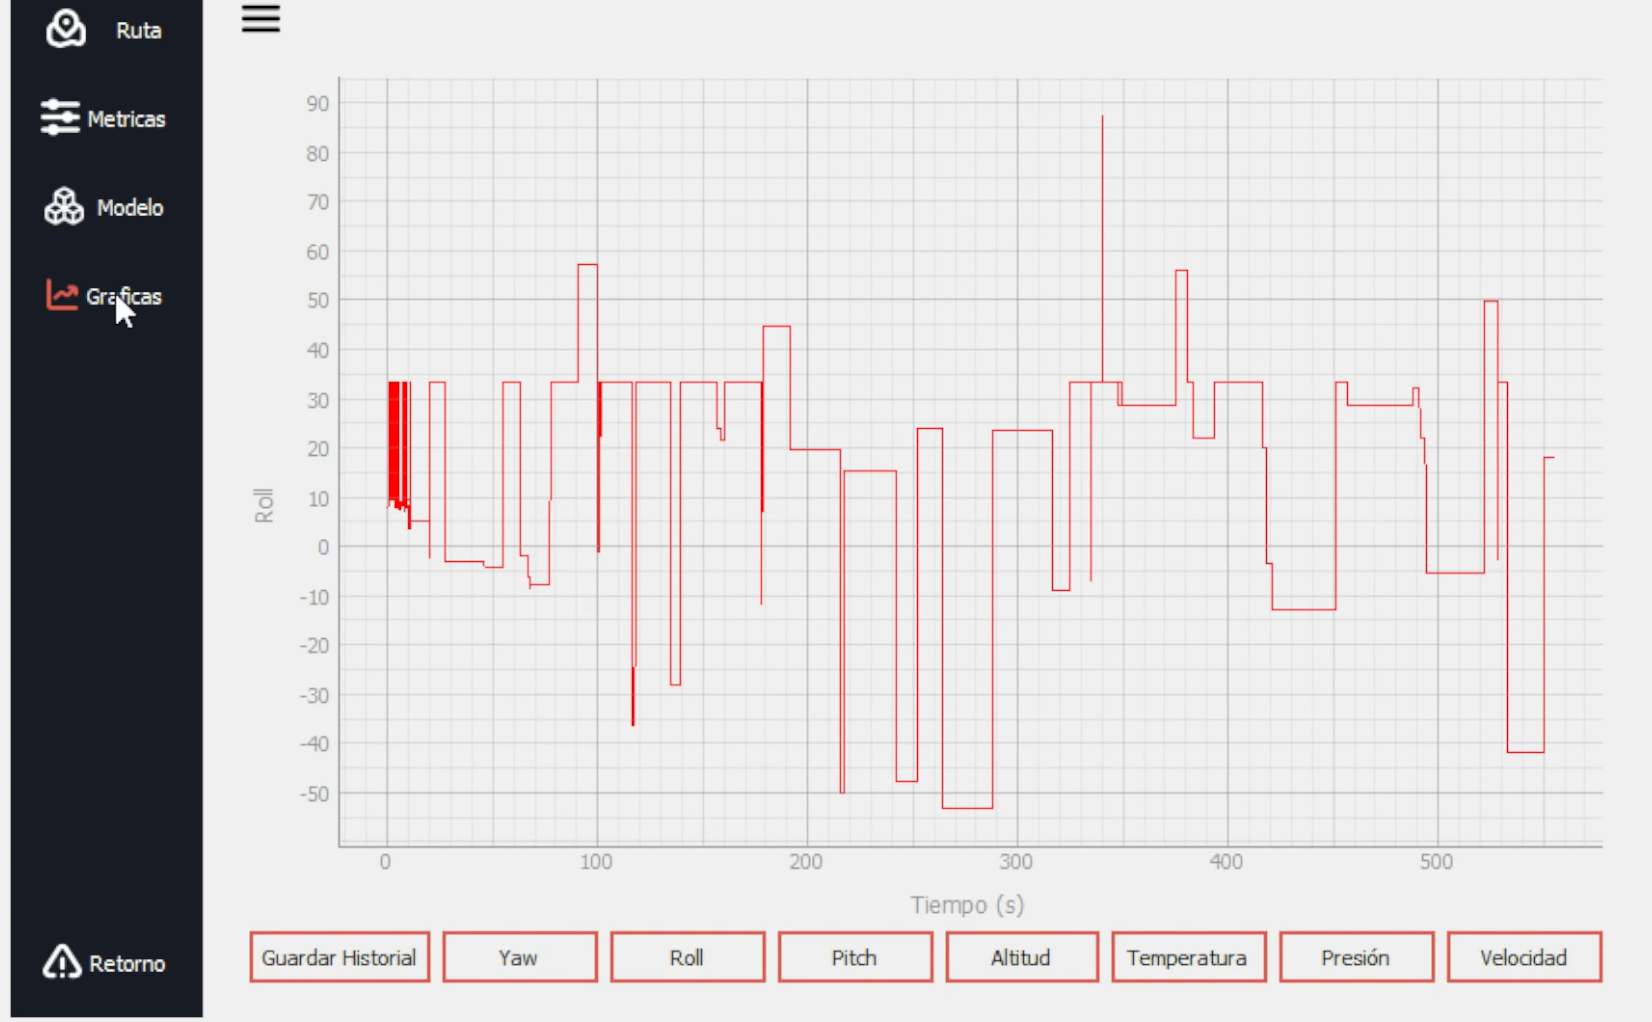
\includegraphics[width=6  in]{Imagenes/Interfaz/graficas.png}
    \caption{Gráficas de funcionamiento UAV }
    \label{fig:graficas }
\end{figure}
